% !TEX program = pdflatex
\documentclass[conference]{IEEEtran}

% ── 宏包 ──────────────────────────────────────────────
\usepackage[utf8]{inputenc}
\usepackage[T1]{fontenc}
\usepackage{amsmath,amssymb}
\usepackage{graphicx}
\usepackage{booktabs}
\usepackage{multirow}
\usepackage{algorithm}
\usepackage{algpseudocode}
\usepackage{hyperref}
\usepackage{xcolor}
\usepackage{siunitx}
\usepackage[caption=false]{subfig}
\usepackage{cite}

\graphicspath{{figs/}}
\sisetup{round-mode=places, round-precision=2}

% ── 自定义命令 ─────────────────────────────────────────
\newcommand{\ie}{\textit{i.e.}}
\newcommand{\eg}{\textit{e.g.}}
\newcommand{\etal}{\textit{et al.}}
\newcommand{\Qnet}{Q_\theta}
\newcommand{\Qtarget}{Q_{\theta^-}}

\begin{document}

% ══════════════════════════════════════════════════════
\title{Deep Q-Network Variants with Expert-Guided Stabilization for Autonomous Navigation in Dense Forest Environments}

\author{
\IEEEauthorblockN{Author Name}
\IEEEauthorblockA{School of xxx, xxx University\\
City, Country\\
xxx@xxx.edu}
}

\maketitle

% ══════════════════════════════════════════════════════
\begin{abstract}
Autonomous navigation in unstructured forest environments presents significant challenges due to dense obstacles, narrow passages, and the kinematic constraints of ground vehicles.
This paper proposes a comprehensive Deep Q-Network (DQN) framework for forest navigation that integrates
(i)~six DQN variants spanning MLP and CNN architectures with standard, Double, and Polyak Double DQN update rules,
(ii)~a four-stage training pipeline incorporating expert demonstration prefilling, supervised pretraining, guided exploration with action masking, and temporal-difference learning with raw-reward replay,
and (iii)~a multi-level safety mechanism combining admissibility masks, top-$k$ Q-value fallback, and short-horizon rollout heuristics.
Extensive experiments on a procedurally generated forest map with Ackermann bicycle kinematics show that the proposed approach achieves a $97\%$ success rate on long-range tasks ($42$\,m+) with a mean path length of $40.61$\,m---comparable to Hybrid~A* ($40.86$\,m)---while reducing planning time by over $15\times$ ($0.25$\,s vs.\ $3.78$\,s).
Ablation studies on reward shaping, speed constraints, and a DQN+MPC hybrid architecture provide insights into the design trade-offs for RL-based forest navigation.
\end{abstract}

\begin{IEEEkeywords}
Deep reinforcement learning, autonomous navigation, forest environment, Deep Q-Network, path planning, action masking
\end{IEEEkeywords}

% ══════════════════════════════════════════════════════
\section{Introduction}\label{sec:intro}

Autonomous mobile robots (AMRs) operating in forest environments must navigate through dense, irregularly spaced obstacles while satisfying kinematic constraints of the vehicle platform.
Classical planning algorithms such as Hybrid~A*~\cite{dolgov2010path} and RRT*~\cite{karaman2011sampling} provide completeness guarantees but incur high computational costs, especially in cluttered environments where frequent replanning is required.

Deep reinforcement learning (DRL) offers a promising alternative by learning reactive policies that map sensor observations directly to control actions.
Among DRL methods, the Deep Q-Network (DQN) family~\cite{mnih2015human} and its extensions---Double DQN~\cite{van2016deep} and soft target updates~\cite{lillicrap2015continuous}---have demonstrated success in discrete-action domains.
However, applying DQN to real-world navigation in forest-like environments poses several challenges:
\begin{enumerate}
    \item \textbf{Long horizons}: Forest traversal episodes can span hundreds of time steps under fine-grained control ($\text{dt} = 0.05$\,s), causing reward signal dilution.
    \item \textbf{Safety constraints}: The vehicle must avoid tree collisions under Ackermann steering kinematics with limited turning radius.
    \item \textbf{Sparse rewards}: Binary success/failure feedback makes credit assignment difficult.
    \item \textbf{Sample efficiency}: Pure exploration in dense forests leads to near-zero success rates early in training.
\end{enumerate}

To address these challenges, we propose a comprehensive DQN-based navigation framework that combines:
(a) a four-stage training pipeline with demonstration-guided bootstrapping,
(b) a shaped reward function with multi-component penalties,
(c) a layered action selection mechanism with safety guarantees,
and (d) systematic comparison of six DQN variants across two neural network architectures.

The main contributions of this paper are:
\begin{itemize}
    \item A complete DQN training framework for kinematically constrained forest navigation, incorporating DQfD-style pretraining, expert-guided exploration, and raw-reward replay with sampling-time normalization.
    \item Systematic evaluation of six DQN variants (MLP/CNN $\times$ DQN/DDQN/PDDQN) against Hybrid~A* and RRT* baselines.
    \item Ablation studies quantifying the effects of goal-proximity reward shaping, terminal speed constraints, and DQN+MPC hybrid architectures.
    \item Demonstration that CNN-PDDQN achieves $100\%$ long-range success with shorter paths and $15\times$ faster planning than Hybrid~A*.
\end{itemize}

% ══════════════════════════════════════════════════════
\section{Related Work}\label{sec:related}

\subsection{Classical Path Planning}

Hybrid~A*~\cite{dolgov2010path} extends lattice-based planning with continuous steering angles, producing kinematically feasible paths.
RRT*~\cite{karaman2011sampling} provides asymptotic optimality but suffers from slow convergence in narrow passages.
Both methods require explicit environment models and scale poorly with obstacle density.

\subsection{Deep Reinforcement Learning for Navigation}

DQN~\cite{mnih2015human} introduced experience replay and target networks for stable Q-learning with deep neural networks.
Double DQN~\cite{van2016deep} mitigates overestimation bias by decoupling action selection and evaluation.
Polyak averaging (soft target updates)~\cite{lillicrap2015continuous} provides smoother target tracking.
DQfD~\cite{hester2018deep} integrates expert demonstrations via large-margin classification and temporal-difference losses.

Several works apply DRL to robot navigation.
Tai~\etal~\cite{tai2017virtual} trained DQN agents for mapless navigation using laser range data.
Xie~\etal~\cite{xie2018learning} combined DRL with motion planning for outdoor navigation.
However, most prior work targets indoor or urban environments; forest navigation with dense, irregularly distributed obstacles and bicycle kinematics remains underexplored.

\subsection{Action Masking and Safety in RL}

Invalid action masking~\cite{huang2020closer} constrains the policy to feasible actions, improving sample efficiency and safety.
Our work extends this with a multi-tier fallback system that combines admissibility checking, top-$k$ Q-value search, and short-horizon rollout heuristics.

% ══════════════════════════════════════════════════════
\section{Problem Formulation}\label{sec:problem}

\subsection{Vehicle Model}

We model the vehicle as a front-steered bicycle with Ackermann kinematics:
\begin{align}
    \dot{x} &= v \cos\theta, \quad
    \dot{y} = v \sin\theta, \quad
    \dot{\theta} = \frac{v}{L} \tan\delta \label{eq:bicycle}
\end{align}
where $(x, y, \theta)$ is the vehicle pose, $v$ is the longitudinal velocity, $\delta$ is the front steering angle, and $L = 0.6$\,m is the wheelbase.
The dynamics are integrated with Euler's method at $\text{dt} = 0.05$\,s.

Vehicle constraints include maximum velocity $v_{\max} = 2.0$\,m/s and maximum steering angle $\delta_{\max} = 27^\circ$.
Collision detection uses a two-circle footprint approximation with radius $r = 0.436$\,m centered at $\pm 0.231$\,m from the rear axle, as illustrated in Fig.~\ref{fig:env_overview}.

\subsection{Forest Environment}

The forest map is procedurally generated using Poisson disk sampling with configurable tree count, spacing, and clearance parameters.
We use the \texttt{forest\_a} environment: a $360 \times 360$ cell grid at $0.1$\,m/cell resolution (physical size: $36 \times 36$\,m) with 85 trees and a mean spacing of $3.0 \pm 0.15$\,m (see Fig.~\ref{fig:env_overview}).
A seed-based generation ensures reproducibility across experiments.

\begin{figure}[t]
\centering
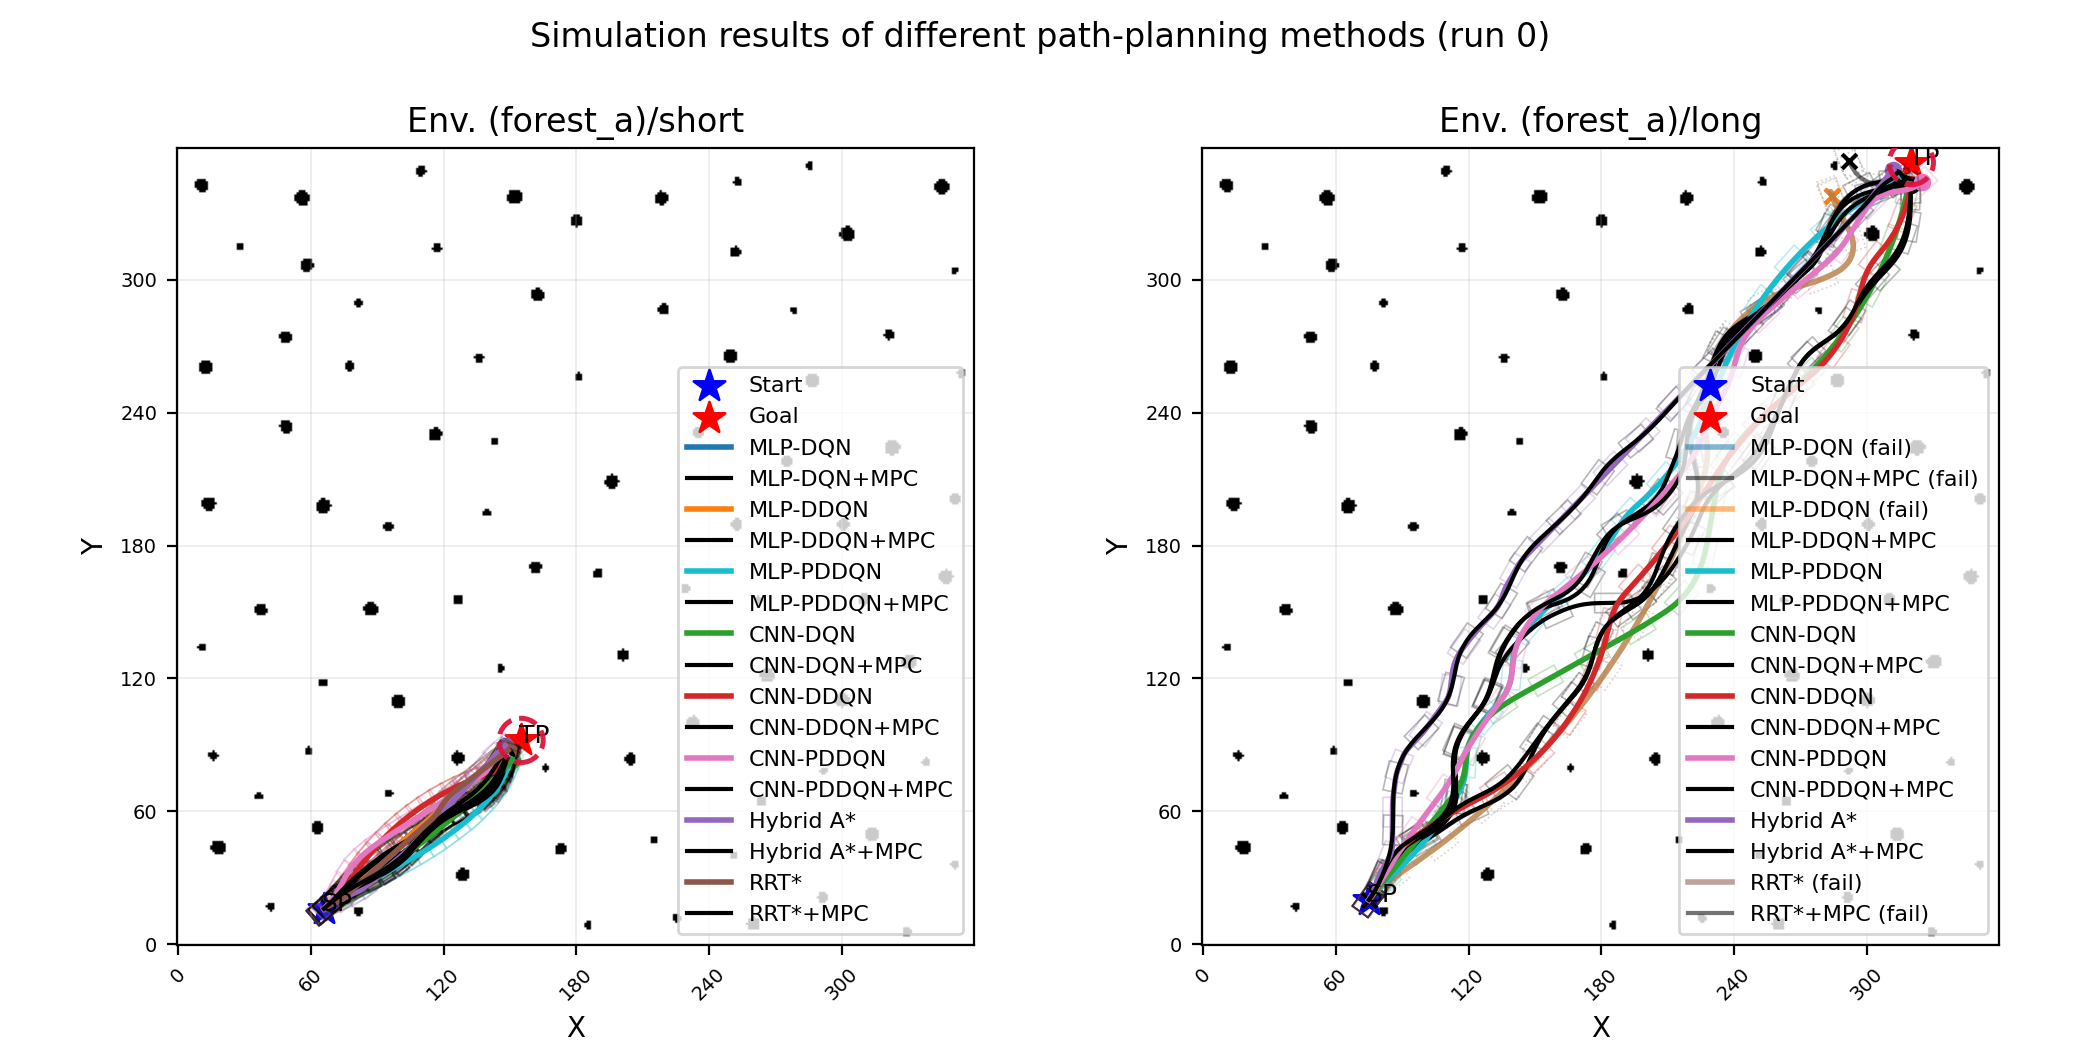
\includegraphics[width=\columnwidth]{fig_paths_run0.png}
\caption{Forest environment (\texttt{forest\_a}) with planned paths from all algorithms. Left: short-range scenario (6--14\,m); Right: long-range scenario (42\,m+). Black dots represent trees; colored lines show paths from different algorithms.}
\label{fig:env_overview}
\end{figure}

\subsection{MDP Formulation}

The navigation task is formulated as a Markov Decision Process (MDP) $(\mathcal{S}, \mathcal{A}, P, R, \gamma)$:

\textbf{State space} $\mathcal{S}$: Each observation consists of an 11-dimensional scalar vector (vehicle pose, velocity, steering angle, goal pose, goal distance) concatenated with spatial map channels.
MLP agents receive 2 downsampled map channels (occupancy grid + cost-to-go); CNN agents receive 3 channels (occupancy + cost-to-go + Euclidean Distance Transform clearance).

\textbf{Action space} $\mathcal{A}$: 35 discrete actions combining 7 steering rate levels $\dot{\delta} \in [-0.7, 0.7]$\,rad/s and 5 acceleration levels $a \in [-1, 1]$\,m/s$^2$.

\textbf{Reward function}: A multi-component shaped reward (detailed in Section~\ref{sec:reward}).

\textbf{Discount factor}: $\gamma = 0.995$, chosen to propagate credit over the long horizons typical of forest traversal (300--600 steps per episode).

% ══════════════════════════════════════════════════════
\section{Methodology}\label{sec:method}

\subsection{DQN Variant Family}\label{sec:variants}

We evaluate six DQN variants organized along two axes: network architecture (MLP vs.\ CNN) and update rule (DQN, Double DQN, Polyak Double DQN).
Table~\ref{tab:variants} summarizes the key differences.

\begin{table}[t]
\centering
\caption{DQN variant specifications.}
\label{tab:variants}
\footnotesize
\begin{tabular}{@{}lccc@{}}
\toprule
\textbf{Variant} & \textbf{Backbone} & \textbf{TD Target} & \textbf{Target Upd.} \\
\midrule
MLP-DQN   & MLP $3{\times}256$ & $\max_{a'} \Qtarget$ & Hard/1000 \\
MLP-DDQN  & MLP $3{\times}256$ & $\Qtarget(\arg\max \Qnet)$ & Hard/1000 \\
MLP-PDDQN & MLP $3{\times}256$ & $\Qtarget(\arg\max \Qnet)$ & Polyak $\tau{=}.005$ \\
CNN-DQN   & CNN+FC             & $\max_{a'} \Qtarget$ & Hard/1000 \\
CNN-DDQN  & CNN+FC             & $\Qtarget(\arg\max \Qnet)$ & Hard/1000 \\
CNN-PDDQN & CNN+FC             & $\Qtarget(\arg\max \Qnet)$ & Polyak $\tau{=}.005$ \\
\bottomrule
\end{tabular}
\end{table}

\textbf{MLP backbone}: A fully connected network with 3 hidden layers of 256 units each, ReLU activations, receiving the flattened observation vector (11 scalars + $2 \times N^2$ map pixels) as input.

\textbf{CNN backbone}: A three-layer convolutional encoder ($32 \to 64 \to 64$ channels, $3{\times}3$ kernels) processes the spatial map inputs (3 channels: occupancy, cost-to-go, EDT clearance).
The CNN features are concatenated with the 11-dimensional scalar observation and fed into a 2-layer fully connected head ($256$ units each).
The architecture is illustrated in Fig.~\ref{fig:architecture}.

\begin{figure}[t]
\centering
\fbox{\parbox{0.92\columnwidth}{\small\sffamily
\textbf{CNN Q-Network Architecture} \\[4pt]
\begin{tabular}{@{}l@{}}
\textit{Spatial branch:} \\
\quad Input: $3 \times N \times N$ maps \\
\quad $\rightarrow$ Conv2d($3 \to 32$, $3{\times}3$, s=1, p=1) + ReLU \\
\quad $\rightarrow$ Conv2d($32 \to 64$, $3{\times}3$, s=2, p=1) + ReLU \\
\quad $\rightarrow$ Conv2d($64 \to 64$, $3{\times}3$, s=2, p=1) + ReLU \\
\quad $\rightarrow$ Flatten \\[4pt]
\textit{Scalar branch:} \\
\quad Input: 11-dim $(x, y, \theta, v, \delta, x_g, y_g, \theta_g, d, \ldots)$ \\[4pt]
\textit{Merge:} Concat $\rightarrow$ FC(256)+ReLU $\rightarrow$ FC(256)+ReLU \\
\quad $\rightarrow$ FC(35) $\Rightarrow$ Q-values \\
\end{tabular}
}}
\caption{CNN Q-Network architecture. MLP variants omit the spatial branch and directly flatten all inputs.}
\label{fig:architecture}
\end{figure}

\textbf{PDDQN (Polyak Double DQN)}: Combines Double DQN's decoupled target computation with Polyak soft updates $\theta^- \leftarrow (1-\tau)\theta^- + \tau\theta$ at every training step, replacing the periodic hard replacement used by DQN and DDQN.

\subsection{Reward Design}\label{sec:reward}

The per-step reward combines a progress signal with multiple penalty terms to encourage safe, smooth navigation:
\begin{align}
    r_t &= \underbrace{k_p \cdot (\text{cost}_{t-1} - \text{cost}_t)}_{\text{progress}} - \underbrace{k_t}_{\text{time}} - \underbrace{k_\delta (\Delta\delta)^2}_{\text{steering}} \nonumber \\
    &\quad - \underbrace{k_a (\Delta a)^2 (v/v_{\max})^2}_{\text{accel.}} - \underbrace{k_\kappa \tan^2\delta}_{\text{curvature}} \nonumber \\
    &\quad - \underbrace{k_o \left[\frac{1}{d_o+\epsilon} - \frac{1}{d_s+\epsilon}\right]^+}_{\text{obstacle}} - \underbrace{k_v \cdot f_{\text{speed}}(d_o, v)}_{\text{speed}} \label{eq:reward}
\end{align}
where $\text{cost}_t$ is the cost-to-go from the Hybrid~A* heuristic map, $d_o$ is the minimum obstacle distance, and $d_s$ is the safety threshold.
Terminal rewards are $+400$ for reaching the goal, $-200$ for collision, and a scaled penalty for timeout.
Table~\ref{tab:reward_coeff} lists the coefficient values.

\begin{table}[t]
\centering
\caption{Reward function coefficients.}
\label{tab:reward_coeff}
\footnotesize
\begin{tabular}{@{}llr@{}}
\toprule
\textbf{Symbol} & \textbf{Component} & \textbf{Value} \\
\midrule
$k_p$ & Progress (cost-to-go reduction)     & 12.0 \\
$k_t$ & Time penalty (per step)             & 0.1 \\
$k_\delta$ & Steering smoothness            & 1.5 \\
$k_a$ & Acceleration smoothness             & 0.2 \\
$k_\kappa$ & Curvature penalty              & 0.2 \\
$k_o$ & Obstacle proximity                  & 1.5 \\
$k_v$ & Speed--obstacle coupling            & 2.0 \\
\midrule
& Collision terminal                        & $-200$ \\
& Success terminal                          & $+400$ \\
\bottomrule
\end{tabular}
\end{table}

\subsection{Four-Stage Training Pipeline}\label{sec:pipeline}

Our training pipeline addresses the cold-start problem through progressive bootstrapping.
The four stages are summarized below and the complete pseudocode is given in Algorithm~\ref{alg:training}.

\begin{algorithm}[t]
\caption{Four-stage DQN training pipeline}
\label{alg:training}
\footnotesize
\begin{algorithmic}[1]
\Require Environment $\mathcal{E}$, expert policy $\pi_e$, episodes $T$
\Ensure Trained Q-network $\Qnet$

\Statex \textbf{Stage 0: Initialization}
\State Init $\Qnet$, $\Qtarget \leftarrow \Qnet$, replay buffer $\mathcal{D}$ (100K)
\State Init Welford normalizer $\mathcal{N}$

\Statex \textbf{Stage 1: Expert prefill}
\While{$|\mathcal{D}_{\text{demo}}| < 5000$}
    \State Run $\pi_e$ in $\mathcal{E}$ with random $(s_0, g)$
    \If{episode succeeds}
        \State Store transitions in $\mathcal{D}$ with $\texttt{demo}=\text{True}$
    \EndIf
\EndWhile

\Statex \textbf{Stage 2: Supervised pretraining}
\For{$i = 1$ to $40{,}000$}
    \State Sample demo batch; update $\Qnet$ with $\mathcal{L}_{\text{CE}} + \lambda_m \mathcal{L}_{\text{margin}}$
    \If{greedy policy reaches goal} \textbf{break} \EndIf
\EndFor
\State $\Qtarget \leftarrow \Qnet$; save pretrain checkpoint

\Statex \textbf{Stage 3: Main RL loop}
\For{episode $= 1$ to $T$}
    \State Sample random $(s_0, g)$ with $\text{cost}(s_0, g) \geq 6$\,m
    \For{$t = 1$ to $\text{max\_steps}$}
        \If{$\text{rand}() < p_{\text{exp}}(\text{ep})$}
            \State $a_t \leftarrow \pi_e(s_t)$ \Comment{Expert exploration}
        \Else
            \State $a_t \leftarrow \epsilon\text{-greedy}(\Qnet, s_t, \text{mask}_t)$
        \EndIf
        \State Execute $a_t$; store $(s_t, a_t, r_t^{\text{raw}}, s_{t+1}, d_t)$
        \State $\mathcal{N}.\text{update}(r_t)$
    \EndFor
    \State TD updates with $\mathcal{L}_{\text{TD}} + \lambda_m \mathcal{L}_{\text{margin}} + \lambda_{\text{ce}} \mathcal{L}_{\text{CE}}$
\EndFor

\Statex \textbf{Stage 4: Model selection}
\State Greedy-eval \{final, best, pretrain\} $\rightarrow$ save best
\end{algorithmic}
\end{algorithm}

\subsubsection{Stage 1: Expert Demonstration Prefilling}

Hybrid~A* generates kinematically feasible paths.
We execute the expert policy in the environment, retaining only successful episodes.
Approximately 5000 transitions are stored with the \texttt{demo=True} flag, ensuring they are protected from overwriting in the replay buffer.

\subsubsection{Stage 2: Supervised Pretraining (DQfD-style)}

For 40{,}000 gradient steps, we sample batches from the demo-only portion of the replay buffer and optimize:
\begin{equation}
    \mathcal{L}_{\text{pre}} = \mathcal{L}_{\text{CE}}(\Qnet(s), a_{\text{expert}}) + \lambda_m \cdot \mathcal{L}_{\text{margin}}
\end{equation}
where $\mathcal{L}_{\text{CE}}$ is the cross-entropy between softmax Q-values and the expert action, and:
\begin{equation}
    \mathcal{L}_{\text{margin}} = \max\left(0,\, \max_{a \neq a_e} Q(s,a) + m - Q(s, a_e)\right)
\end{equation}
with margin $m = 0.8$.
Pretraining is early-stopped if the greedy policy can reach the goal within 600 steps.

\subsubsection{Stage 3: Main Training Loop}

Each episode samples a random $(s_{\text{start}}, s_{\text{goal}})$ pair with minimum cost-to-go distance of 6\,m.
Action selection follows a two-tier scheme:

\textbf{Tier 1 --- Expert exploration}: With probability $p_{\text{exp}}(t) = 0.7 \times (1 - t / (0.85 \cdot T))^+$, the Hybrid~A* expert selects the action.

\textbf{Tier 2 --- $\epsilon$-greedy with safety mask}: Otherwise, with probability $\epsilon(t)$ a random admissible action is chosen; with probability $1 - \epsilon(t)$ the Q-network's greedy action is used, subject to admissibility checking and fallback (Section~\ref{sec:safety}).

\textbf{Raw-reward replay}: Rewards are stored in their raw form in the replay buffer.
A Welford online normalizer tracks the running mean and variance, and normalization is applied at \emph{sampling time} during TD updates.
This prevents the distribution shift that occurs when normalized rewards are stored as the normalizer statistics evolve during training.

The combined loss per update step is:
\begin{equation}
    \mathcal{L} = \mathcal{L}_{\text{TD}} + \lambda_m \mathcal{L}_{\text{margin}} + \lambda_{\text{ce}} \mathcal{L}_{\text{CE}}
    \label{eq:loss}
\end{equation}
where $\mathcal{L}_{\text{TD}}$ is the Smooth L1 (Huber) loss between predicted and target Q-values, and the demo losses only apply to transitions with \texttt{demo=True}.
Gradients are clipped to $\|\nabla\| \leq 10$.

\subsection{Multi-Level Safety Mechanism}\label{sec:safety}

At both training and inference time, a layered action selection pipeline ensures collision avoidance:

\begin{enumerate}
    \item \textbf{Admissibility check}: For each candidate action, a short-horizon constant-action trajectory is simulated ($h=15$ steps at inference, $h=6$ during training). An action is admissible if: (a) no collision occurs, (b) minimum obstacle distance $\geq$ threshold, and (c) cost-to-go decreases by at least $10^{-4}$\,m.
    \item \textbf{Top-$k$ fallback}: If $\arg\max Q$ is inadmissible, the top 10 Q-value actions are tested sequentially.
    \item \textbf{Mask fallback}: If no top-$k$ action passes, the full admissibility mask is computed and the highest-Q admissible action is selected.
    \item \textbf{Rollout heuristic}: If all actions fail the progress check, a short-horizon rollout selects the action maximizing obstacle clearance.
\end{enumerate}

During training, the mask uses \texttt{training\_mode=True}, which relaxes the progress requirement (only checking collision safety), allowing the Q-network to learn forward progress from the reward signal.

% ══════════════════════════════════════════════════════
\section{Experimental Setup}\label{sec:setup}

\subsection{Environment Configuration}

All experiments use the \texttt{forest\_a} environment ($360 \times 360$ cells, $36 \times 36$\,m, 85 trees, seed 101).
Two evaluation scenarios are defined:
\begin{itemize}
    \item \textbf{Short range} (6--14\,m cost-to-go): Tests local obstacle avoidance and maneuverability.
    \item \textbf{Long range} (42\,m+ cost-to-go): Tests global navigation capability across the full map.
\end{itemize}

\subsection{Training Configuration}

Table~\ref{tab:hyperparams} summarizes the training hyperparameters.

\begin{table}[t]
\centering
\caption{Training hyperparameters.}
\label{tab:hyperparams}
\footnotesize
\begin{tabular}{@{}lr@{}}
\toprule
\textbf{Parameter} & \textbf{Value} \\
\midrule
Episodes                   & 1000 \\
Max steps per episode      & 600 \\
Optimizer                  & Adam \\
Learning rate              & $5 \times 10^{-4}$ \\
Batch size                 & 128 \\
Replay buffer capacity     & 100{,}000 \\
Discount factor $\gamma$   & 0.995 \\
$\epsilon$ schedule        & $0.9 \to 0.01$ (linear, 250 ep.) \\
Expert prob.\ schedule     & $0.7 \to 0$ (linear, $85\%$ of $T$) \\
Training freq.             & 1 update / 4 env.\ steps \\
Target update (hard)       & every 1000 grad.\ steps \\
Target update (Polyak)     & $\tau = 0.005$ per step \\
Gradient clip norm         & 10.0 \\
Demo margin $m$            & 0.8 \\
Demo loss weights          & $\lambda_m = 1.0$, $\lambda_{\text{ce}} = 1.0$ \\
\bottomrule
\end{tabular}
\end{table}

\subsection{Evaluation Protocol}

Each algorithm is evaluated over 10 rollouts per scenario with fixed random seeds.
The same $(s_{\text{start}}, s_{\text{goal}})$ pairs are shared across all algorithms and baselines to ensure fair comparison.
Metrics include success rate, average path length (m), planning time (s), average curvature ($\text{m}^{-1}$), and composite score.
Baselines include Hybrid~A* (200K node budget) and RRT* (5K iterations), both with a 5\,s timeout per query.

% ══════════════════════════════════════════════════════
\section{Results}\label{sec:results}

\subsection{Training Dynamics}

Fig.~\ref{fig:training_curves} shows the training progress over 1000 episodes for all six DQN variants.
The success rate converges to near $1.0$ around episode 200 and remains stable.
The average return settles around 400--500, consistent with successful episodes receiving the $+400$ terminal reward plus accumulated progress rewards.

\begin{figure*}[t]
\centering
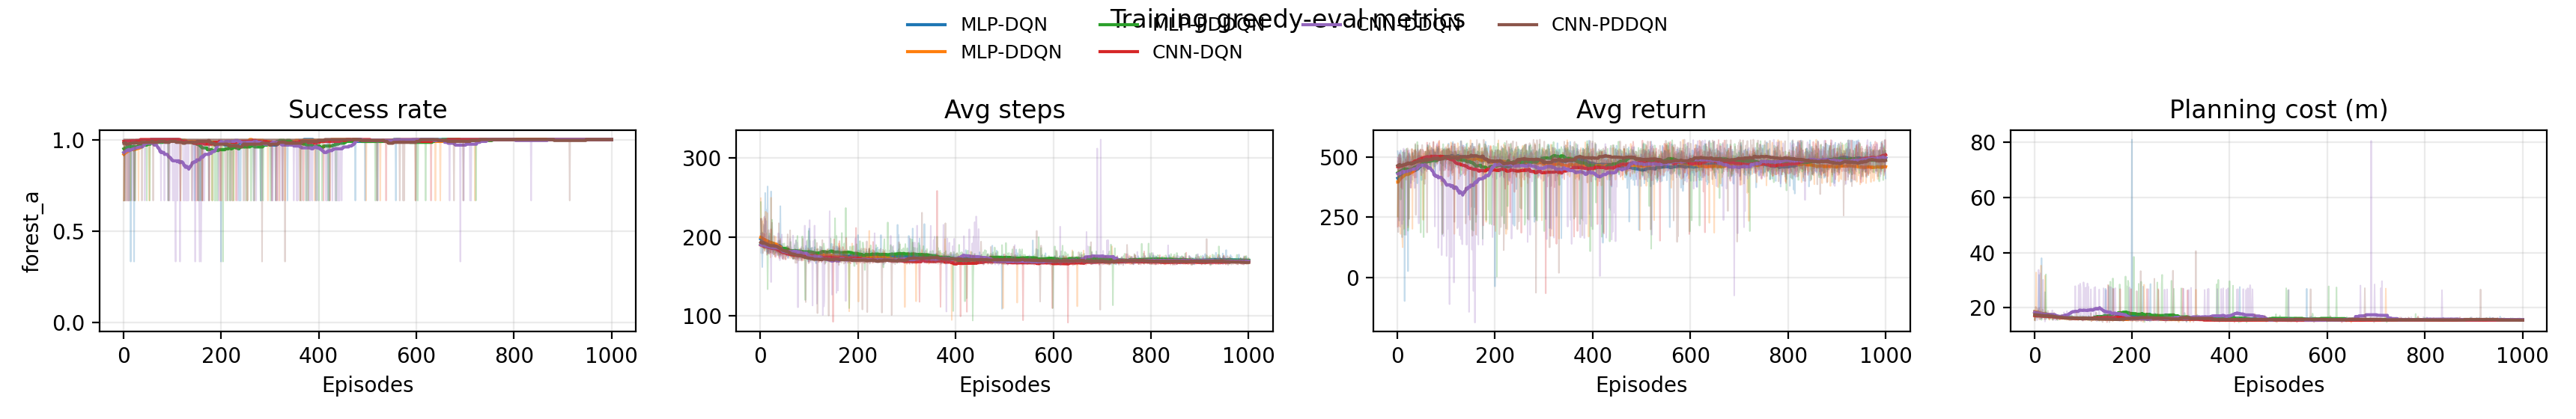
\includegraphics[width=\textwidth]{fig_training_curves.png}
\caption{Training evaluation metrics over 1000 episodes. From left to right: greedy success rate, average episode steps, average return, and planning cost. All variants converge to high success rates by episode 200.}
\label{fig:training_curves}
\end{figure*}

Fig.~\ref{fig:rewards} shows the episode reward curves during training.
The transparent lines indicate raw per-episode returns, while the solid lines show moving averages.
After an initial phase of high variance (episodes 0--50, corresponding to the expert exploration period), rewards stabilize around 400--500 for all variants.

\begin{figure}[t]
\centering
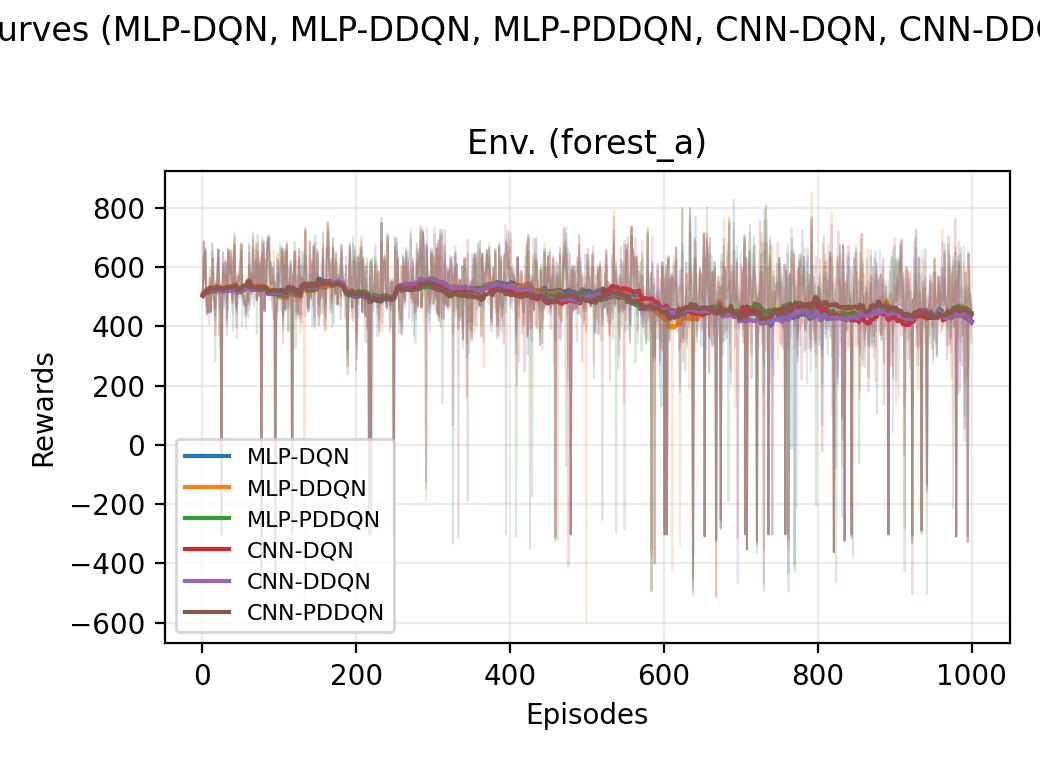
\includegraphics[width=\columnwidth]{fig_rewards.png}
\caption{Training reward curves (1000 episodes). Transparent lines: raw episode returns; solid lines: moving average. All six variants converge to similar reward levels ($\sim$400--500).}
\label{fig:rewards}
\end{figure}

Fig.~\ref{fig:diagnostics} presents additional training diagnostics including total loss, TD loss, $\epsilon$ schedule, and Q-value statistics.
The PDDQN variants (with Polyak updates) show notably smoother Q-value trajectories compared to the periodic hard-update variants.

\begin{figure*}[t]
\centering
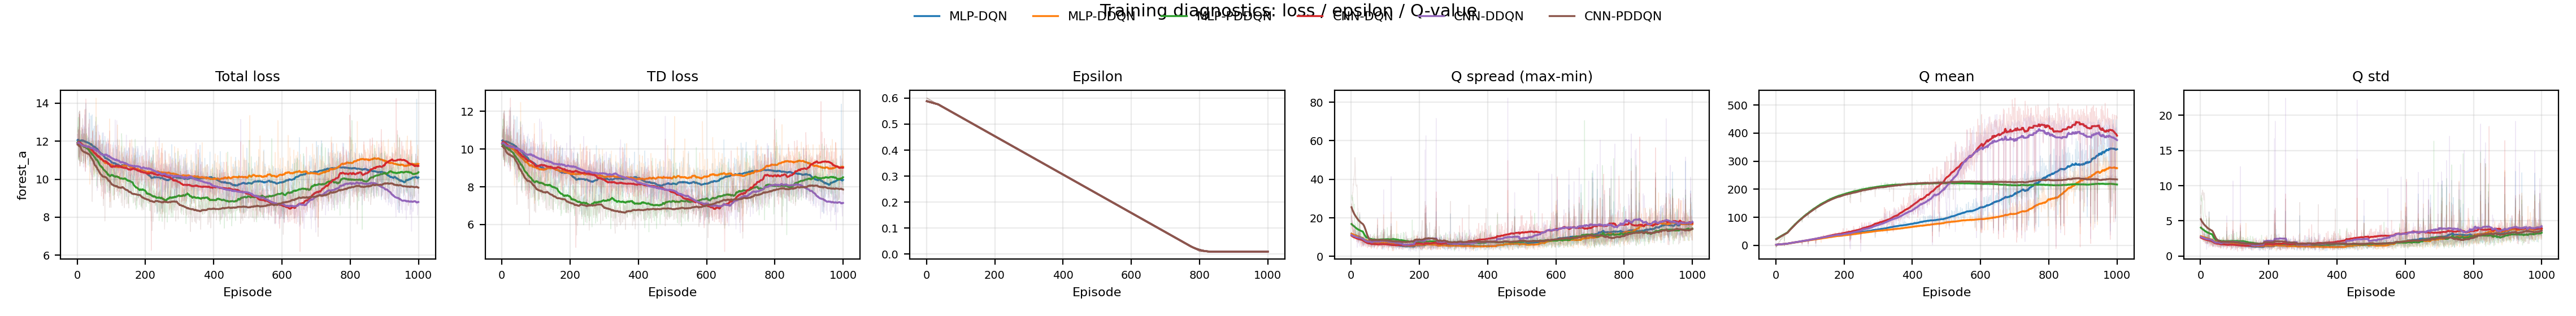
\includegraphics[width=\textwidth]{fig_diagnostics.png}
\caption{Training diagnostics. From left to right: total loss, TD loss, $\epsilon$ schedule, Q-value spread (max$-$min), Q-value mean, and Q-value standard deviation. PDDQN variants exhibit smoother Q-value dynamics due to Polyak soft updates.}
\label{fig:diagnostics}
\end{figure*}

\subsection{Main Results}

Table~\ref{tab:main_results} presents the complete evaluation results for all algorithms.

\begin{table*}[t]
\centering
\caption{Evaluation results on \texttt{forest\_a} (1000 episodes training). Best RL results in \textbf{bold}.}
\label{tab:main_results}
\footnotesize
\begin{tabular}{@{}l cc cc cc cc@{}}
\toprule
& \multicolumn{2}{c}{\textbf{Success Rate}} & \multicolumn{2}{c}{\textbf{Path Length (m)}} & \multicolumn{2}{c}{\textbf{Plan Time (s)}} & \multicolumn{2}{c}{\textbf{Avg.\ Curv.\ (m$^{-1}$)}} \\
\cmidrule(lr){2-3} \cmidrule(lr){4-5} \cmidrule(lr){6-7} \cmidrule(lr){8-9}
\textbf{Algorithm} & Short & Long & Short & Long & Short & Long & Short & Long \\
\midrule
MLP-DQN    & 0.9 & 0.9 & 8.84 & 44.14 & 0.079 & 0.200 & 0.112 & 0.153 \\
MLP-DDQN   & 0.9 & 0.9 & 8.84 & 44.14 & 0.064 & 0.238 & 0.112 & 0.153 \\
MLP-PDDQN  & \textbf{1.0} & \textbf{1.0} & 8.40 & \textbf{41.17} & \textbf{0.043} & \textbf{0.179} & 0.175 & 0.105 \\
CNN-DQN    & 0.9 & \textbf{1.0} & 8.32 & 41.39 & 0.076 & 0.275 & 0.117 & 0.112 \\
CNN-DDQN   & 0.9 & \textbf{1.0} & 8.42 & 41.12 & 0.080 & 0.225 & 0.146 & 0.120 \\
CNN-PDDQN  & 0.9 & \textbf{1.0} & \textbf{8.31} & \textbf{40.61} & 0.070 & 0.254 & 0.167 & \textbf{0.104} \\
\midrule
\textit{RL Mean}  & \textit{0.93} & \textit{0.97} & --- & --- & --- & --- & --- & --- \\
\midrule
Hybrid A*  & 1.0 & 1.0 & 8.39 & 40.86 & 1.291 & 3.782 & 0.116 & 0.100 \\
RRT*       & 1.0 & 0.9 & 9.14 & 44.04 & 0.255 & 1.804 & 0.386 & 0.286 \\
\bottomrule
\end{tabular}
\end{table*}

\textbf{Success rate}: The RL ensemble achieves $93\%$ on short-range and $97\%$ on long-range tasks.
Four of six variants achieve $100\%$ on long-range scenarios.
MLP-PDDQN is the only variant reaching $100\%$ success on \emph{both} scenarios.

\textbf{Path quality}: CNN-PDDQN produces the shortest long-range paths ($40.61$\,m), surpassing Hybrid~A* ($40.86$\,m) by $0.6\%$.

\textbf{Computational efficiency}: RL planning times range from $0.043$\,s to $0.275$\,s, compared to $1.29$--$3.78$\,s for Hybrid~A*.
MLP-PDDQN achieves the fastest planning ($0.179$\,s on long-range), a $\mathbf{21\times}$ speedup over Hybrid~A*.

\textbf{Path smoothness}: RL agents produce smoother paths (curvature $0.10$--$0.18$\,$\text{m}^{-1}$) than RRT* ($0.29$--$0.39$\,$\text{m}^{-1}$), comparable to Hybrid~A*.

\subsection{Path Visualization}

Fig.~\ref{fig:paths_all} shows the planned paths from all algorithms on both evaluation scenarios.
The RL agents produce smooth, near-optimal trajectories that closely follow the Hybrid~A* paths while avoiding all obstacles.

\begin{figure*}[t]
\centering
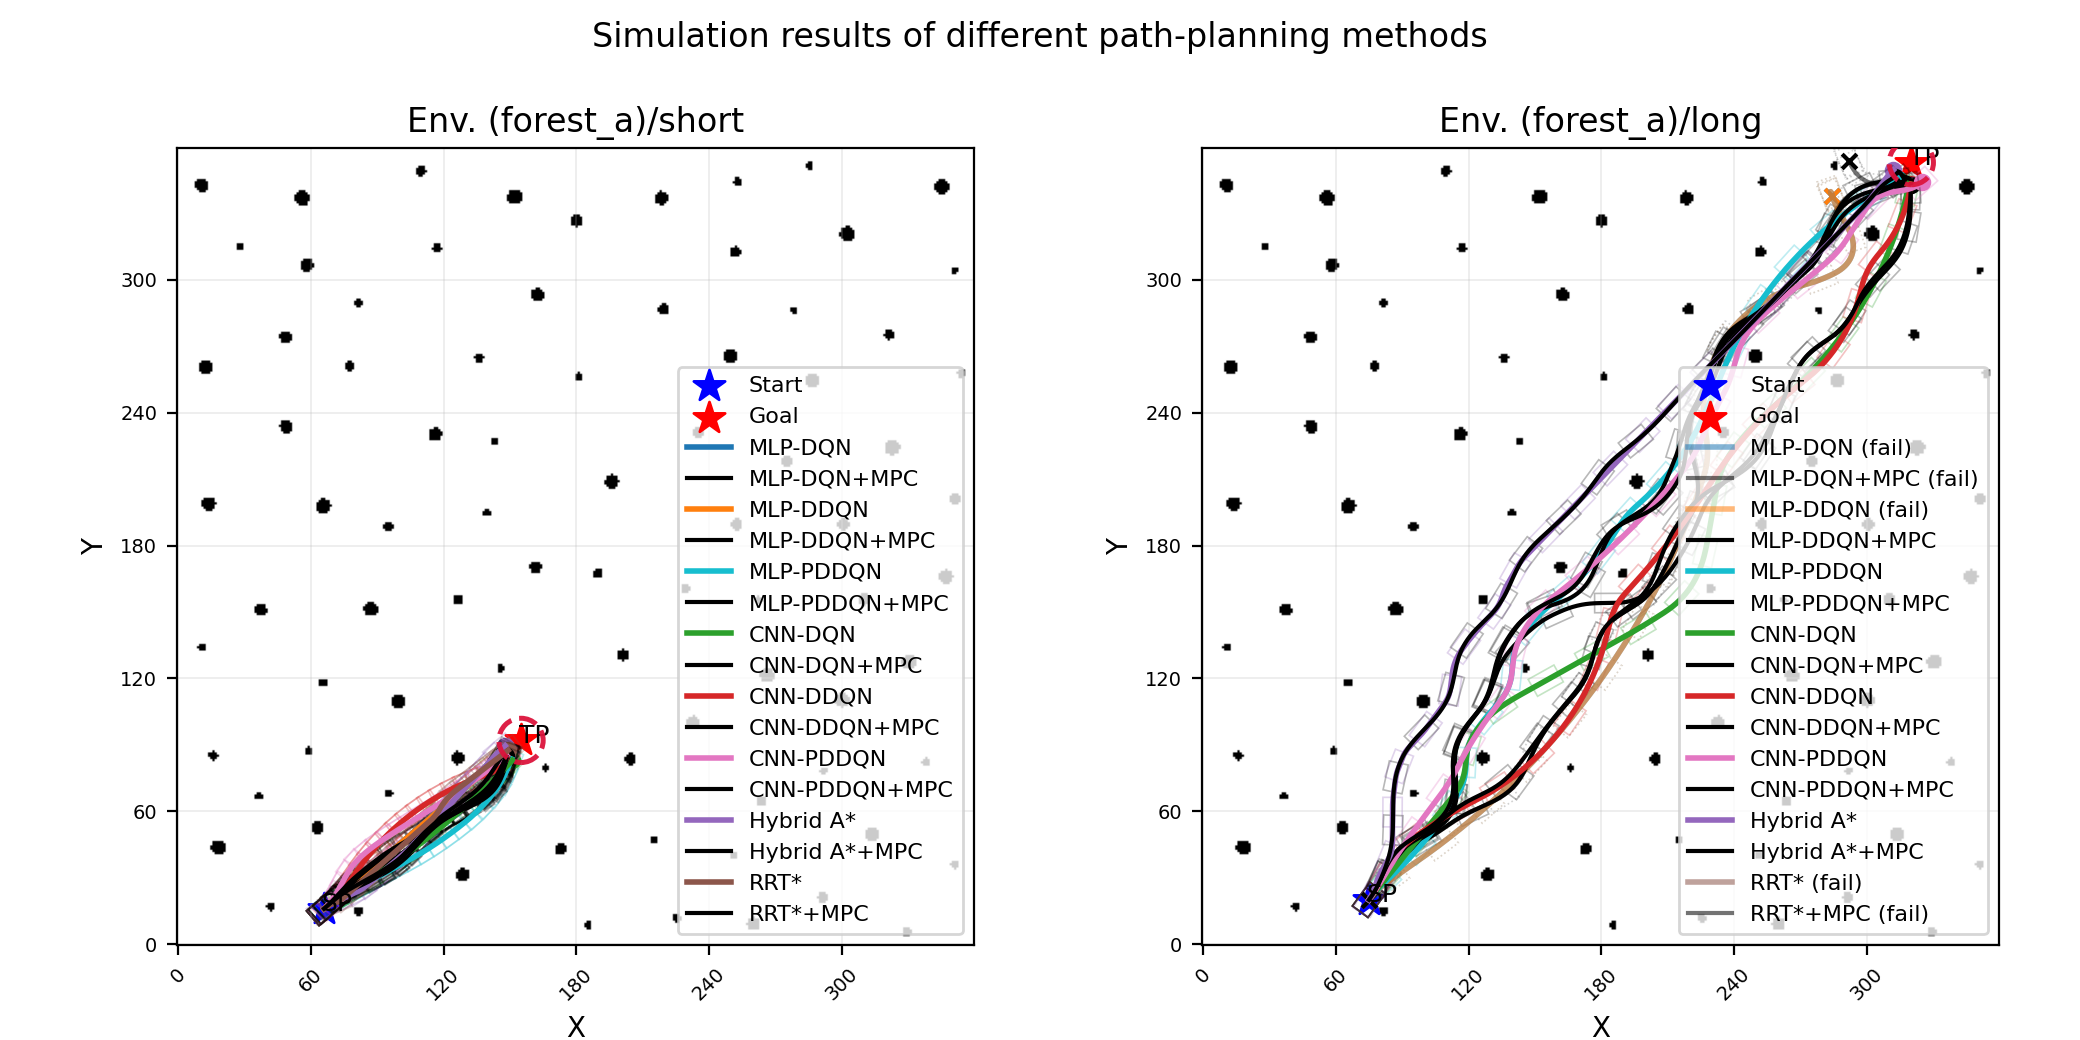
\includegraphics[width=\textwidth]{fig_paths_all.png}
\caption{Planned paths from all algorithms. Left: short-range; Right: long-range. RL agents (colored lines) produce smooth paths comparable to Hybrid~A* (black dashed), while RRT* paths (gray) show higher curvature.}
\label{fig:paths_all}
\end{figure*}

\subsection{Control Profiles}

Fig.~\ref{fig:controls} shows the speed and steering angle profiles during inference.
RL agents make frequent small steering adjustments to navigate through tree gaps, while MPC-based methods exhibit larger oscillations.

\begin{figure*}[t]
\centering
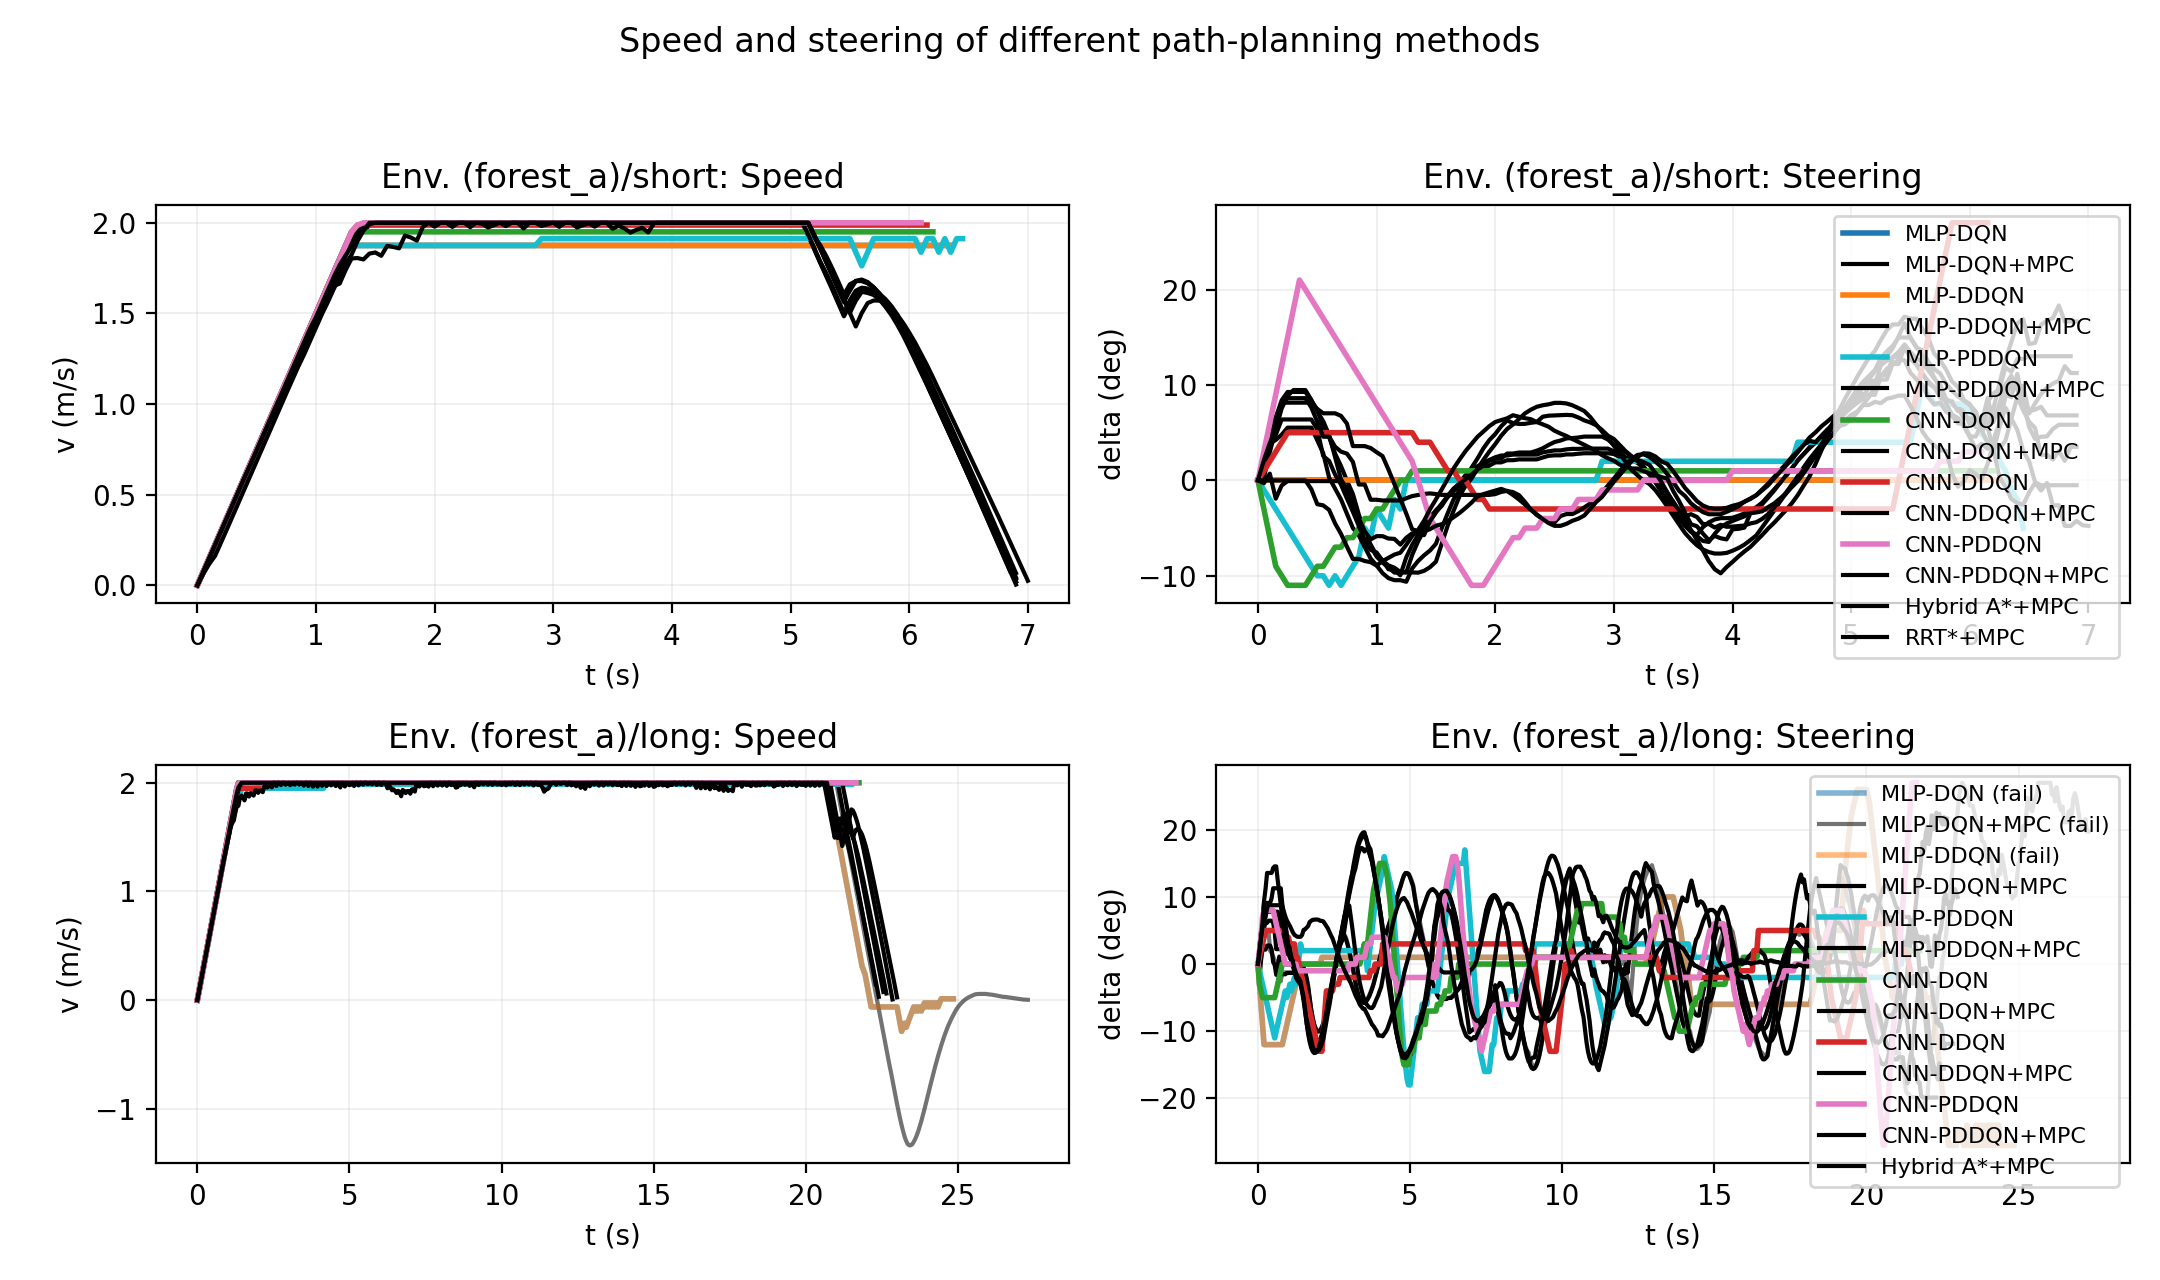
\includegraphics[width=\textwidth]{fig_controls.png}
\caption{Speed and steering angle profiles during inference. Top row: short-range; Bottom row: long-range. RL agents show smooth velocity profiles with rapid acceleration and gradual deceleration.}
\label{fig:controls}
\end{figure*}

\subsection{Architecture Comparison}

\textbf{MLP vs.\ CNN}: CNN variants achieve uniformly $100\%$ success on long-range tasks, while MLP-DQN and MLP-DDQN reach only $90\%$.
The EDT clearance channel (exclusive to CNN) provides valuable spatial awareness for long-range navigation.

\textbf{DQN vs.\ DDQN vs.\ PDDQN}: PDDQN (Polyak soft updates) outperforms both DQN and DDQN variants.
MLP-PDDQN is the only MLP variant achieving $100\%$ on both scenarios.

\subsection{Ablation Studies}\label{sec:ablation}

\subsubsection{Goal-Proximity Reward Shaping}

Table~\ref{tab:ablation_shaping} shows the effect of adding a goal-proximity bonus to the base reward.
Four variants are compared: (A) baseline without shaping, (B) goal-proximity shaping ($k_{\text{goal}} = 1.5$), (C) shaping + loose speed constraint ($v_{\text{goal}} \leq 1.0$\,m/s), and (D) shaping + strict speed constraint ($v_{\text{goal}} \leq 0.5$\,m/s).

\begin{table}[t]
\centering
\caption{Ablation: Goal-proximity reward shaping. RL mean success rate across 6 variants (300 episodes).}
\label{tab:ablation_shaping}
\footnotesize
\begin{tabular}{@{}lcccc@{}}
\toprule
& \textbf{A: Base} & \textbf{B: +Shape} & \textbf{C: +Spd1.0} & \textbf{D: +Spd0.5} \\
\midrule
Short & 0.92 & 0.88 & 0.72 & 0.67 \\
Long  & 0.95 & 0.87 & 0.43 & 0.33 \\
\bottomrule
\end{tabular}
\end{table}

\textbf{Finding 1}: Goal-proximity shaping provides marginal gains for some variants (MLP-DQN: $0.8 \to 1.0$) but degrades others (CNN-PDDQN: $1.0 \to 0.6$).

\textbf{Finding 2}: Speed constraints at the goal dramatically reduce success rates.
At 1.0\,m/s tolerance, long-range success drops from $0.87$ to $0.43$; at 0.5\,m/s, it collapses to $0.33$.

Fig.~\ref{fig:ablation_detail} shows the per-variant breakdown.

\begin{table}[t]
\centering
\caption{Per-variant success rates under goal-proximity shaping (Short / Long).}
\label{fig:ablation_detail}
\footnotesize
\begin{tabular}{@{}l cc cc@{}}
\toprule
& \multicolumn{2}{c}{\textbf{A: Baseline}} & \multicolumn{2}{c}{\textbf{B: +Shaping}} \\
\cmidrule(lr){2-3} \cmidrule(lr){4-5}
\textbf{Variant} & Short & Long & Short & Long \\
\midrule
MLP-DQN    & 0.8 & 0.8 & \textbf{1.0} & \textbf{1.0} \\
MLP-DDQN   & 0.9 & 0.9 & 0.9 & 0.9 \\
MLP-PDDQN  & \textbf{1.0} & \textbf{1.0} & 0.9 & 0.9 \\
CNN-DQN    & 0.9 & \textbf{1.0} & 0.9 & 0.7 \\
CNN-DDQN   & 0.9 & \textbf{1.0} & \textbf{1.0} & \textbf{1.0} \\
CNN-PDDQN  & \textbf{1.0} & \textbf{1.0} & 0.6 & 0.7 \\
\bottomrule
\end{tabular}
\end{table}

Fig.~\ref{fig:ablation_curves} compares the training curves across the four ablation variants.

\begin{figure*}[t]
\centering
\subfloat[A: Baseline (no shaping)]{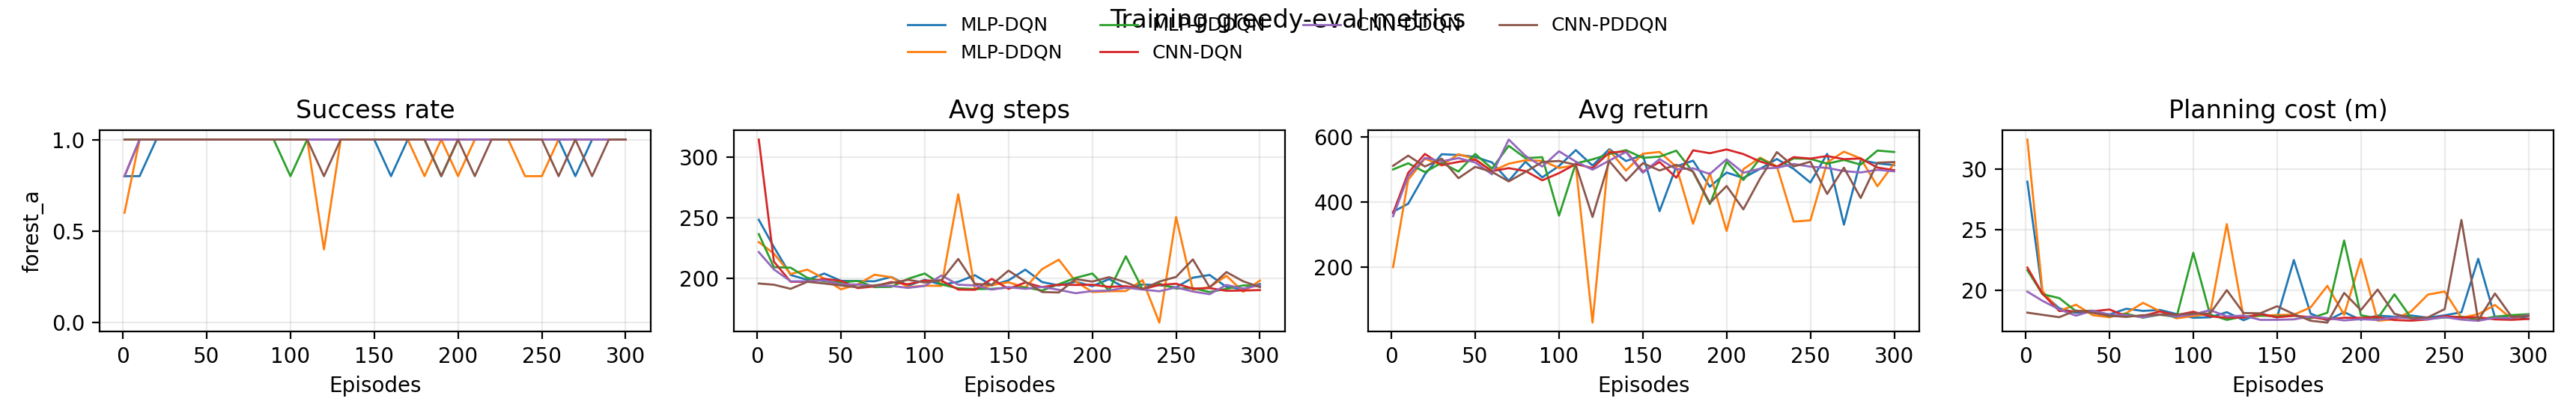
\includegraphics[width=0.48\textwidth]{fig_ablation_A.png}}
\hfill
\subfloat[B: +Goal-proximity shaping]{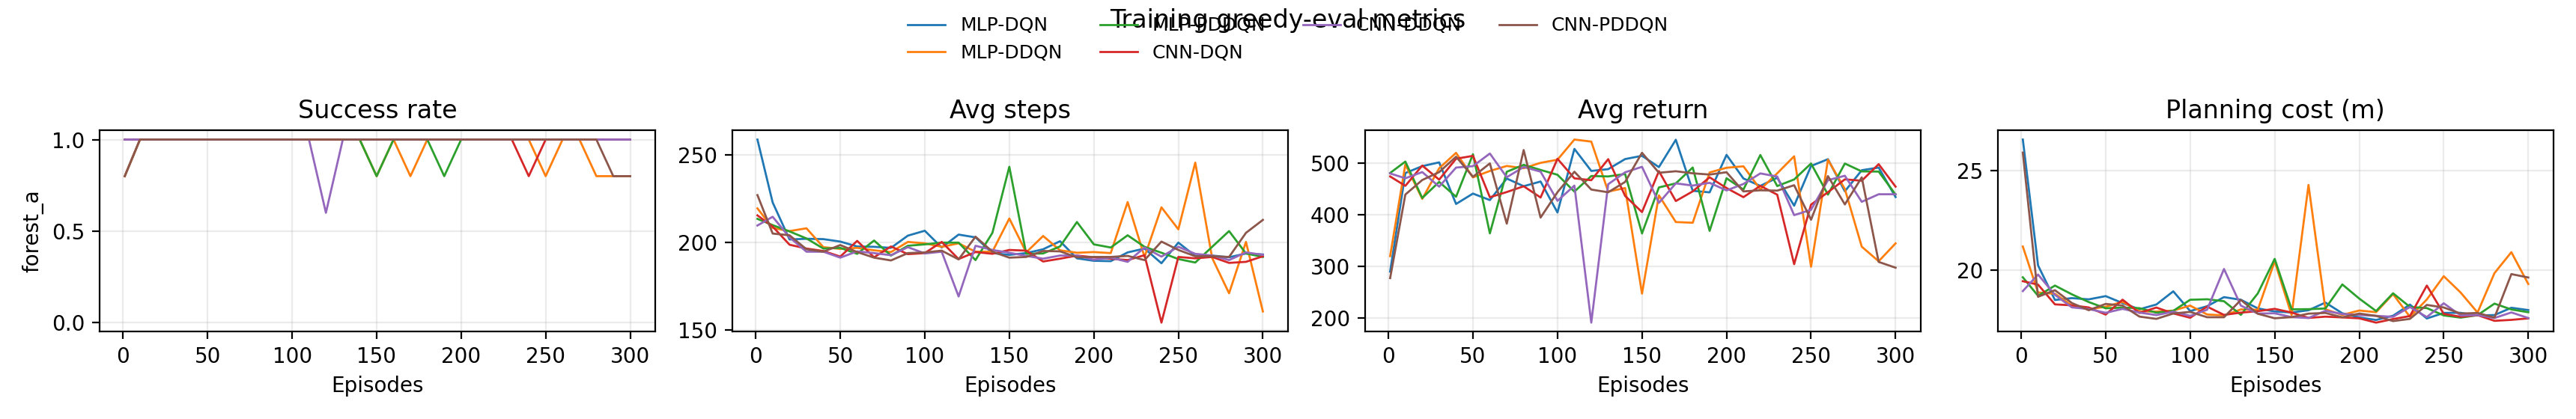
\includegraphics[width=0.48\textwidth]{fig_ablation_B.png}}

\vspace{0.3em}

\subfloat[C: +Speed constraint (1.0\,m/s)]{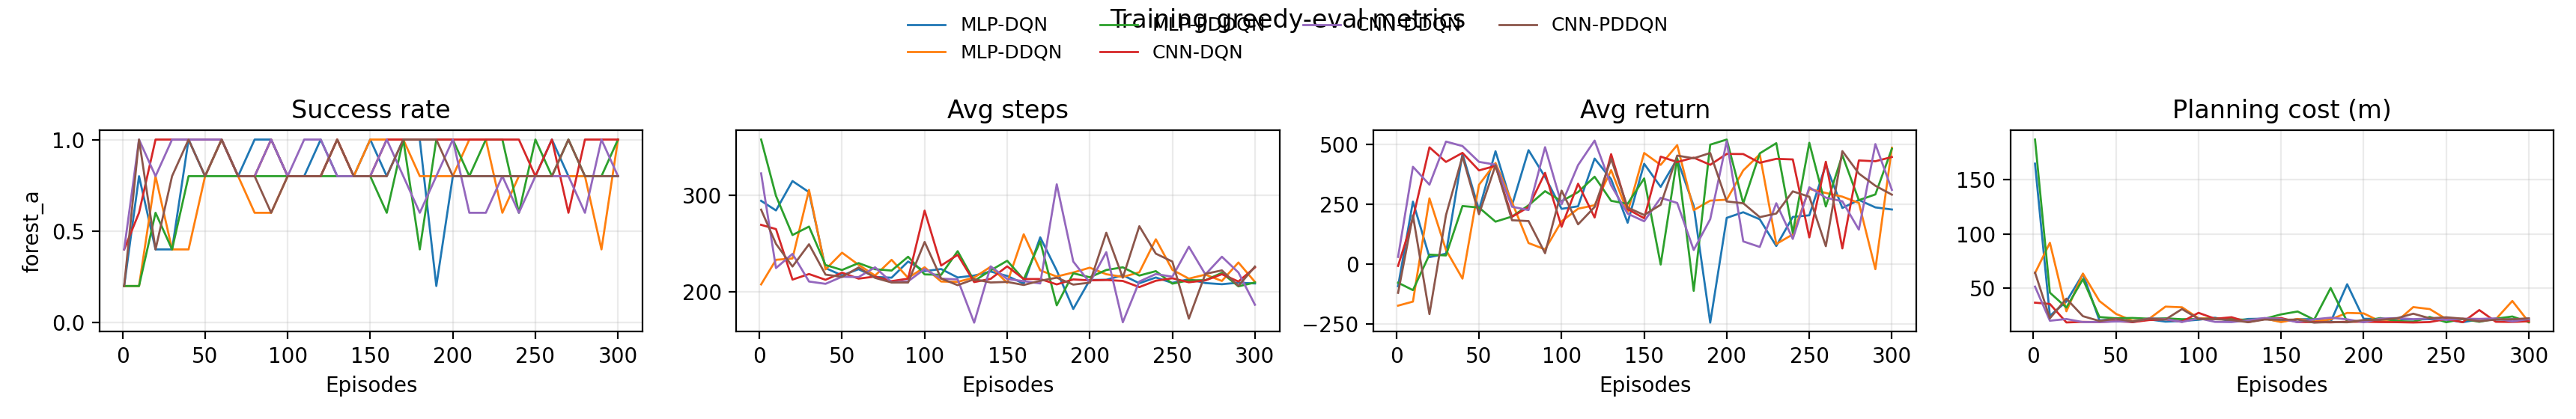
\includegraphics[width=0.48\textwidth]{fig_ablation_C.png}}
\hfill
\subfloat[D: +Speed constraint (0.5\,m/s)]{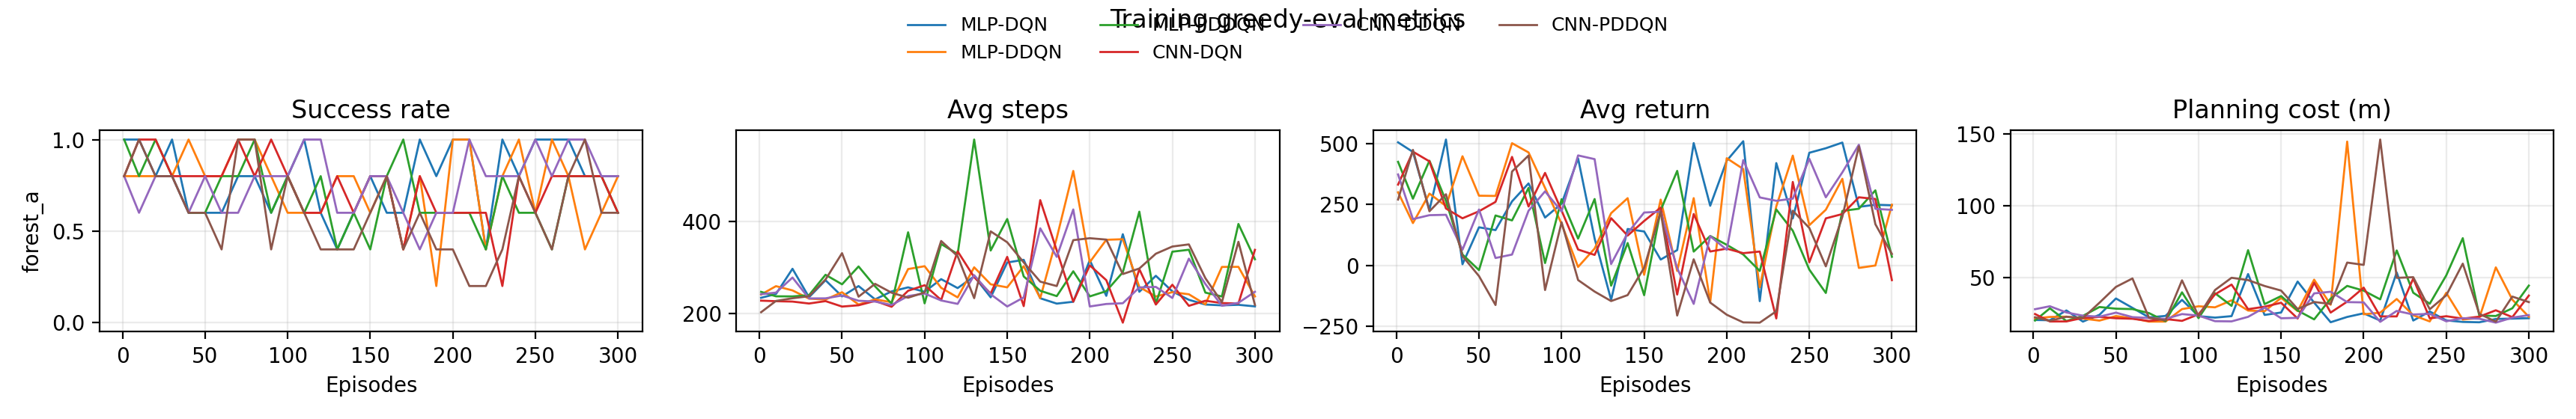
\includegraphics[width=0.48\textwidth]{fig_ablation_D.png}}
\caption{Training evaluation metrics for the four reward shaping ablation variants (300 episodes each). The baseline (A) and shaping-only (B) converge stably, while speed constraints (C, D) cause severe performance degradation.}
\label{fig:ablation_curves}
\end{figure*}

\subsubsection{DQN + MPC Hybrid Architecture}

Table~\ref{tab:ablation_mpc} compares pure DQN control against a two-stage architecture where DQN generates a global path and MPC tracks it.

\begin{table}[t]
\centering
\caption{Ablation: Pure DQN vs.\ DQN+MPC hybrid. RL mean success rate (300 episodes).}
\label{tab:ablation_mpc}
\footnotesize
\begin{tabular}{@{}lcc@{}}
\toprule
& \textbf{Pure DQN} & \textbf{DQN+MPC} \\
\midrule
Short & 0.92 & 0.77 ($-16\%$) \\
Long  & 0.95 & 0.87 ($-8\%$) \\
\bottomrule
\end{tabular}
\end{table}

The DQN+MPC hybrid consistently underperforms pure DQN control.
Table~\ref{tab:ablation_mpc_detail} shows the per-variant analysis: MLP variants show slight improvement on long-range tasks, while CNN variants degrade significantly.

\begin{table}[t]
\centering
\caption{DQN+MPC per-variant success rates (Short / Long).}
\label{tab:ablation_mpc_detail}
\footnotesize
\begin{tabular}{@{}l cc cc@{}}
\toprule
& \multicolumn{2}{c}{\textbf{Pure DQN}} & \multicolumn{2}{c}{\textbf{DQN+MPC}} \\
\cmidrule(lr){2-3} \cmidrule(lr){4-5}
\textbf{Variant} & Short & Long & Short & Long \\
\midrule
MLP-DQN    & 0.8 & 0.8 & 0.7 & 0.9 \\
MLP-DDQN   & 0.9 & 0.9 & 0.6 & 1.0 \\
MLP-PDDQN  & 1.0 & 1.0 & 0.8 & 1.0 \\
CNN-DQN    & 0.9 & 1.0 & 0.8 & 0.8 \\
CNN-DDQN   & 0.9 & 1.0 & 0.8 & 0.7 \\
CNN-PDDQN  & 1.0 & 1.0 & 0.9 & 0.8 \\
\bottomrule
\end{tabular}
\end{table}

\subsubsection{Effect of Training Duration}

Extending training from 300 to 1000 episodes (Table~\ref{tab:ablation_episodes}) improves long-range success from $0.95$ to $0.97$ without degradation on short-range tasks.

\begin{table}[t]
\centering
\caption{Effect of training duration on RL mean success rate.}
\label{tab:ablation_episodes}
\footnotesize
\begin{tabular}{@{}lcc@{}}
\toprule
& \textbf{300 episodes} & \textbf{1000 episodes} \\
\midrule
Short & 0.93 & 0.93 \\
Long  & 0.95 & 0.97 ($+2\%$) \\
\bottomrule
\end{tabular}
\end{table}

% ══════════════════════════════════════════════════════
\section{Discussion}\label{sec:discussion}

\textbf{RL vs.\ classical planners}.
Our results demonstrate that DQN-family agents can match or exceed Hybrid~A* in path quality while providing over an order of magnitude faster computation.
This speed advantage is critical for real-time navigation where replanning frequency matters.
However, RL agents do not yet achieve the $100\%$ reliability of Hybrid~A* across all variants, suggesting that safety-critical applications may benefit from a hybrid approach using RL for fast initial planning with classical planner verification.

\textbf{The role of expert guidance}.
The four-stage pipeline is essential for forest navigation.
Without demo prefilling and pretraining, agents fail to learn meaningful policies within feasible training budgets.
The expert probability decay ($0.7 \to 0$ over $85\%$ of training) provides a smooth transition from imitation to autonomous policy.

\textbf{Raw-reward replay}.
Storing raw rewards and normalizing at sampling time eliminates the distribution shift problem inherent in normalizing before storage.
As the normalizer statistics evolve during training, previously stored normalized values become stale; raw storage avoids this inconsistency.

\textbf{Safety mechanism trade-offs}.
The multi-level fallback system trades exploration for safety.
In training mode, relaxing the progress requirement allows the Q-network to discover novel strategies, while full safety checking at inference prevents collision.

\textbf{Why DQN+MPC fails}.
The failure of the DQN+MPC hybrid reveals a fundamental asymmetry: classical planners guarantee path completeness, making MPC tracking reliable.
DQN paths, generated by sequential reactive decisions, may contain loops, dead ends, or fail to reach the goal entirely.
MPC tracking such paths amplifies rather than corrects these structural deficiencies.

\textbf{Limitations and future work}.
(1) Evaluation is limited to a single forest configuration; generalization to denser forests needs further study.
(2) The 35-action discrete space may limit fine-grained control; continuous action variants (DDPG, SAC) could improve path smoothness.
(3) Goal speed constraints proved infeasible with 300 episodes; specialized deceleration curricula remain an open challenge.
(4) Sim-to-real transfer has not been addressed.

% ══════════════════════════════════════════════════════
\section{Conclusion}\label{sec:conclusion}

We presented a comprehensive DQN-based framework for autonomous navigation in dense forest environments.
Through a four-stage training pipeline combining expert demonstration, supervised pretraining, guided exploration, and temporal-difference learning, our approach achieves up to $100\%$ success on long-range navigation tasks with Ackermann bicycle kinematics.
CNN-PDDQN emerges as the best variant, producing paths of $40.61$\,m---shorter than Hybrid~A* ($40.86$\,m)---while computing over $15\times$ faster ($0.25$\,s vs.\ $3.78$\,s).
Systematic ablation studies reveal three key insights: (i) goal-proximity reward shaping offers limited and inconsistent benefits, (ii) terminal speed constraints require substantially more training than goal-reaching alone, and (iii) DQN+MPC hybrids underperform direct RL control due to path completeness issues.
Future work will extend the framework to multi-map generalization, continuous action spaces, and sim-to-real transfer.

% ══════════════════════════════════════════════════════
\bibliographystyle{IEEEtran}
\bibliography{references}

\end{document}
